\documentclass[10pt]{beamer}
\usetheme{metropolis}
% all imports
\usepackage[utf8]{inputenc}
\usepackage[T1]{fontenc}
\usepackage{lmodern}
\usepackage{appendixnumberbeamer}
\usepackage{hyperref}
\usepackage{booktabs}
\usepackage{bm}
\usepackage[scale=2]{ccicons}
\usepackage[outputdir=build]{minted}
\usepackage{pgfplots}
\usepackage{array,colortbl,xcolor}
\usepgfplotslibrary{dateplot}
\usepackage{setspace}
\usepackage{etoolbox}
\usepackage{xspace}
\usepackage{tikz}
\usetikzlibrary{shapes,arrows,positioning,fit,backgrounds}
\usepackage{tkz-euclide}
\usepackage{soul}
\usepackage{ragged2e}
\usepackage{algorithm}
\usepackage[noend]{algpseudocode}
\usepackage{caption}
\usepackage{amsmath}
\title{Apresentação_Anytime Dynamic A*}

\AtBeginEnvironment{quote}{\singlespacing}

% new commands
\newcommand{\themename}{\textbf{\textsc{metropolis}}\xspace}
\newcommand{\vect}[1]{\bm{#1}}
\newcommand{\myprime}[1]{{#1}^{\prime}}
\newcommand{\grad}[2]{\nabla_{#1} {#2}}
\newcommand{\dotp}[2]{{#1}^{\top}{#2}}
\newcommand{\dotpPright}[2]{{#1}^{\top}\left({#2}\right)}
\newcommand{\outerp}[2]{\left({#1}\right){#2}^{\top}}
\newcommand{\Jacobian}[2]{\frac{\partial #1}{\partial #2}}
\newcommand{\Vocab}{\mathbb{V}}
\DeclareMathOperator*{\argmin}{arg\,min}

% Quote with author reference at the end
\let\oldquote\quote
\let\endoldquote\endquote
\renewenvironment{quote}[2][]
  {\if\relax\detokenize{#1}\relax
     \def\quoteauthor{#2}%
   \else
     \def\quoteauthor{#2~---~#1}%
   \fi
   \oldquote}
  {\par\nobreak\smallskip\hfill(\quoteauthor)%
   \endoldquote\addvspace{\bigskipamount}}
%-----------------------------------------   
% Justifying itemize
% \let\olditem\item
% \renewcommand\item{\olditem\justifying}
%----------------------------------------- 
% Change default caption of algorithm environment
\DeclareCaptionFormat{myformat}{#3}
\captionsetup[algorithm]{format=myformat}
%----------------------------------------- 
% Enables line numbering in any order
\newcommand{\setalglineno}[1]{%
  \setcounter{ALG@line}{\numexpr#1-1}}
  
\algnewcommand\And{\textbf{AND}}
\algnewcommand\Or{\textbf{OR}}
\renewcommand{\algorithmicloop}{\textbf{forever}}

\newlength\myindent
\setlength\myindent{2em}
\newcommand\bindent{%
  \begingroup
  \setlength{\itemindent}{\myindent}
  \addtolength{\algorithmicindent}{\myindent}
}
\newcommand\eindent{\endgroup}

% definitions 
\definecolor{blue}{RGB}{159, 192, 176}
\definecolor{green}{RGB}{160, 227, 127}
\definecolor{orange}{RGB}{243, 188, 125}
\definecolor{red}{RGB}{253, 123, 84}
\definecolor{nephritis}{RGB}{39, 174, 96}
\definecolor{emerald}{RGB}{46, 204, 113}
\definecolor{turquoise}{RGB}{39, 174, 96}
\definecolor{green-sea}{RGB}{22, 160, 133}
% Tikzstyles for Computation Graphs

% nodes
\tikzstyle{noop} = [circle, draw=none, fill=red, minimum size = 10pt]
\tikzstyle{op} = [circle, draw=red, line width=1.5pt, fill=red!70, text=black, text centered, font=\bf \normalsize, minimum size = 25pt]
\tikzstyle{state} = [circle, draw=blue, line width=1.5pt, fill=blue!70, text=black, text centered, font=\bf \normalsize, minimum size = 25pt]
% \tikzstyle{gradient} = [circle, draw=green, line width=1.5pt, fill=green!60, text=black, text centered, font=\bf \normalsize, minimum size = 25pt]
\tikzstyle{gradient} = [circle, draw=nephritis, line width=1.5pt, fill=nephritis!60, text=black, text centered, font=\bf \normalsize, minimum size = 25pt]
\tikzstyle{textonly} = [draw=none, fill=none, text centered, font=\bf \normalsize]
\tikzstyle{boxtextonly} = [draw=none, fill=none, align=center, font=\bf \normalsize]

% edges
% \tikzstyle{tedge}  = [draw, thick, >=stealth, ->]
\tikzstyle{tedge}  = [draw, thick, >=latex, ->]

% namedscope
\tikzstyle{namedscope} = [circle, draw=orange, line width=1.5pt, fill=orange!60, align=center, inner sep=0pt]

% \tikzstyle{container} = [draw=none, rectangle, dotted, inner ysep=1.5em]
% \tikzstyle{novertex} = [draw=none, fill=none, text centered]
% \tikzstyle{predicate} = [ellipse, draw, thick, text centered, rounded corners, minimum size=30pt]
% \tikzstyle{aux} = [rectangle, draw, thick, text centered, rounded corners, minimum size=30pt]
% \tikzstyle{ledge}  = [draw, dashed, thick, >=stealth, ->]
% \tikzstyle{pedge}  = [draw, thick, >=stealth, ->]



\title{Anytime Dynamic A*: \\
\Large An Anytime Replanning Algorithm} 
\date{\today}
\author{Autores: Maxim Likhachev, Dave Ferguson, Geoff Gordon, Anthony Stentz e Sebastian Thrun\\
\\Paula Moraes}
\institute{\textbf{IME-USP}: Instituto de Matemática e Estatística - Universidade de São Paulo}

\titlegraphic{
            \hspace{9cm}
            
\includegraphics[scale=0.2]{images/liamflogo.png}
}



\begin{document}
\nocite{likhachev2005anytime}
\graphicspath{ {images/} }

\maketitle

\section{Introdução}

\begin{frame}{Proposta}
\justify
\begin{itemize}
\item Apresentar um algoritmo de planejamento e replanejamento que seja capaz de produzir soluções subótimas em qualquer momento e ajustar a busca conforme a  entrada de novas informações sobre o domínio.
\vspace{1cm}
\item Combinar as técnicas de \alert{replanejamento} e \alert{algoritmos anytime}, a fim de encontrar soluções para problemas de busca complexos e dinâmicos.
\end{itemize}
\end{frame}

\begin{frame}{Motivação}
O mundo real é inerentemente \textbf{incerto} e \textbf{dinâmico}!
\begin{itemize}
\item modelos precisos e estáticos usados por um planejador, podem rapidamente ficar desatualizados com a realidade
\item operações no mundo físico geralmente possuem um tempo de deliberação limitado 
\item poucos estudos sobre a interação das áreas de replanejamento e algoritmos anytime, sendo que ambas as áreas possuem características que atenderiam às situações complexas e dinâmicas do mundo real
\end{itemize}
\hspace{5cm}
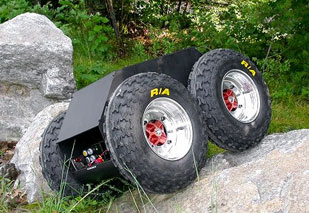
\includegraphics[width=5cm,height=3cm]{rmp.jpg} 
\end{frame}

\begin{frame}{Técnicas atuais}
\begin{exampleblock}{Replanejamento: \textit{D* (Dynamic A*) e \textit{D* Lite}}}
\begin{itemize}
\item Lidam com informações falhas e ambientes dinâmicos, mantendo e incrementando soluções sem a necessidade de gerá-las do zero
\end{itemize}
\end{exampleblock}
\vspace{0.5cm}
\begin{exampleblock}{Anytime: \textit{ARA* (Anytime Reparing A*)}}
\begin{itemize}
\item Abordagem ideal para planejamento sob um tempo restrito, a qual inicialmente devolve uma solução subótima e passa a melhorar esta solução com o restante de tempo disponível
\end{itemize}
\end{exampleblock}
\end{frame}

\section{Replanejamento Incremental}

\begin{frame}{Replanejamento Incremental}
A necessidade de replanejar um caminho pode decorrer da dinâmica e observabilidade parcial de um ambiente. \\
\newline É fundamental que um agente possa planejar novos caminhos ótimos até a meta ao explorar um ambiente desconhecido.
\vspace{0.3cm}
\begin{exampleblock}{A* vs D* Lite}
\begin{itemize}
\item[] \textbf{A*} não atualiza os custos caso haja mudanças no ambiente, nesse caso todo o cálculo é perdido e a busca reiniciada.
\item[] \textbf{D* Lite} mantém os dados dos caminhos calculados e atualiza os custos com a chegada de uma nova informação
\end{itemize}
\end{exampleblock} 
\end{frame}

\begin{frame}{Características D* Lite}
\begin{itemize}
\item Uso eficiente de heurísticas e atualizações incrementais dos resultados de buscas passadas
\vspace{0.5cm}
\item Garantia de otimalidade em busca em grafo
\vspace{0.5cm}
\item Mantém uma lista de caminhos de menor custo entre o estado atual e os estados meta, além do custo dos arcos entre tais estados
\vspace{0.5cm}
\item Guarda uma lista com um custo de um estado $s$ até a meta e o custo de um \textit{lookahead} de um passo $rhs(s)$
\end{itemize}
\end{frame}

\begin{frame}{Características D* Lite}
\begin{equation*}
  rhs(s) =
    \begin{cases}
      0 & \text{if}\:\: s = s_{goal}\\
      min_{s' \in Succ(s)}(c(s,s') + g(s')) & \text{otherwise}
    \end{cases}       
\end{equation*}
Um estado $s$ é \textbf{consistente} sse $g(s) = rhs(s)$\\
\hspace*{2.2cm} \textbf{menos consistente} se $g(s) < rhs(s)$\\
\hspace*{2.2cm} \textbf{mais consistente} se $g(s) > rhs(s)$ \\
\hspace*{2.2cm} \alert{inconsistente} se $g(s) \neq rhs(s)$
\begin{equation*}
\begin{aligned}
key(s) ={} & [k_1(s), k_2(s)] \\
      ={} & [min(g(s), rhs(s)) + h(s_{start}, s), \\
      & min(g(s), rhs(s))] 
\end{aligned}
\end{equation*}
A fila de prioridade OPEN mantém apenas os estados inconsistentes que precisam ser atualizados e feitos localmente consistentes. Resolvendo a consistência desses estados é possível rastrear o menor caminho entre o estado inicial e a meta.
\end{frame}
\begin{frame}{Restrições de tempo}
\textbf{E no caso de situações em que aguardar por uma solução ótima é inviável?} 
\begin{center}

\includegraphics[width=6cm,height=6cm]{robby.png}
\end{center}
\end{frame}

\section{Planejamento Anytime}

\begin{frame}{Algoritmos Anytime}
Dependendo do domínio, nem sempre uma solução ótima é ideal, como é o caso de problemas de planejamento complexos e com tempo limitado. \\
\newline Tais situações requerem uma solução que possa ser gerada no tempo de computação disponível. \\
\newline \alert{Algoritmos anytime} operam sob o \textit{tradeoff} de agilidade sobre otimalidade  \\
\newline \justifying Algoritmos Anytime baseados no A* tem a propriedade de que se a heurística adotada é consistente e os valores da heurística são multiplicados por um fator de multiplicação $\epsilon > 1$, então o custo da solução gerada é garantidamente $\epsilon$ vezes o custo da solução ótima 
\end{frame}

\begin{frame}{Anytime A*}
\begin{itemize}
\item Em muitos domínios multiplicar o valor das heurísticas \textit{weighted} A* (WA*), acelera o tempo de planejamento
\vspace{3px}
\item A solução inicial é produzida rapidamente dentro de um limite alto de subotimalidade e melhorada dentro do tempo restante
\vspace{3px}
\item Usa a noção de consistência entre as buscas, apenas considerando estados cujos custos na busca anterior \textbf{poderiam estar inválidos} dados o novo \textbf{$\epsilon$}
\vspace{3px}
\item Inicia com uma busca A* e \textbf{expande cada estado no máximo uma vez}, caso fique inconsistente na próxima busca, é adicionado a lista INCONS
\vspace{3px}
\item O conteúdo da lista INCONS ao final de uma busca é inserida numa nova fila de prioridade já com os pesos atualizados por \textbf{$\epsilon$} para a próxima busca  
\end{itemize}
\end{frame}

\section{Anytime Dynamic A*}
\begin{frame}{Explicação em alto nível AD*}
\begin{itemize}
\item Realiza uma série de de buscas usando um fator de multiplicação decrescente para gerar uma série de soluções com limites aprimorados (tendendo à otimalidade), como no \alert{ARA*}
\vspace{0.5cm}
\item Quando ocorrem mudanças no ambiente que afetam diretamente o custo das arestas no grafo, estados \textbf{localmente} afetados são colocados na fila de prioridade OPEN e ordenados pelo mínimo entre o novo e o antigo valor $key$, como em \alert{D*}
\vspace{0.5cm}
\item Os estados na fila são processados até que a solução seja certamente $\epsilon$-subótima
\end{itemize}
\end{frame}

\begin{frame}{Detalhes algoritmo}
\begin{itemize}
\item O valor inicial do fator de multiplicação $\epsilon_0$ é suficientemente grande para garantir que uma solução subótima será gerada rapidamente
\vspace{1cm}
\item Se o custo das arestas for alterado significativamente, o algoritmo aumentará o valor de $\epsilon$ a fim de que uma solução subótima possa ser encontrada rapidamente 
\end{itemize}
\end{frame}

\begin{frame}{Algoritmo - AD*}
\begin{algorithm}[H]
\caption{key(s)}
\begin{algorithmic}[1]
\If {$g(s) > rhs(s)$}
\State \textbf{return} [$rhs(s) + \epsilon \cdot h(s_{start}, s); rhs(s)$];
\Else
\State \textbf{return} [$g(s) + h(s_{start}, s); g(s)$];
\EndIf
\end{algorithmic}
\end{algorithm}
\begin{algorithm}[H]
\caption{UpdateState(s)}
\begin{algorithmic}[1]
\setalglineno{5}
\If {$s$ was not visited before}
    \State $g(s) = \infty$;
\EndIf
\If {($s \neq s_{goal}$)} $rhs(s)=min_{s' \in Succ(s)}(c(s,s') + g(s'));$
\EndIf
\If {($s \in OPEN$)} remove $s$ from OPEN;
\EndIf
\If {($g(s) \neq rhs(s)$)} 
  \If {$s \notin CLOSED$}
    \State insert $s$ into OPEN with $key(s)$;
    \Else
    \State insert $s$ into INCONS;
    \EndIf
\EndIf
\end{algorithmic}
\end{algorithm}
\end{frame}

\begin{frame}{Algoritmo - AD* função ComputeOrImprovePath}
\begin{algorithm}[H]
\caption{ComputeOrImprovePath()}
\begin{algorithmic}[1]
\setalglineno{5}
\While {($min_{s \in OPEN}(key(s)) < key(s_{start}) \:\Or\: rhs(s_{start}) \neq  g(s_{start}) $)}
\State remove state $s$ with the minimum key from OPEN;
\If {($g(s) > rhs(s)$)}
\State $g(s) = rhs(s)$;
\State CLOSED = CLOSED $\cup \{s\}$;
\For {\textbf{all} $s' \in Pred(s)$} $UpdateState(s')$;
\EndFor
\Else 
\State $g(s) = \infty$;
\For {\textbf{all} $s' \in Pred(s) \cup \{s\}$} $UpdateState(s')$;
\EndFor
\EndIf
\EndWhile
\end{algorithmic}
\end{algorithm}
\end{frame}

\begin{frame}{Algoritmo - AD* função Main I}
\begin{algorithm}[H]
\caption{Main()}
\begin{algorithmic}[1]
\State $g(s_{start}) = rhs(s_{start}) = \infty$;
\State $\:g(s_{goal}) = \infty$;
\State $rhs(s_{goal}) = 0$; 
\State $\:\epsilon = \epsilon_0$;
\State OPEN = CLOSED = INCONS = $\emptyset$;
\State insert $s_{goal}$ into OPEN with $key(s_{goal})$;
\State $ComputeOrImprovePath()$;
\State publish current $\epsilon$-suboptimal solution;
\Loop
\If {changes in edge costs are detected}
\For {\textbf{all} directed graphs $(u, v)$ with changed edge costs}
\State Update the edge cost $c(u, v)$;
\State $UpdateState(u)$;
\EndFor
\EndIf
\If {significant edge cost changes were observed}
\State increase $\epsilon$ or replan from scratch;
\Else \If {$\epsilon > 1$}
\State decrease $\epsilon$;
\EndIf
\EndIf
\EndLoop
\end{algorithmic}
\end{algorithm}
\end{frame}

\begin{frame}{Algoritmo - AD* função Main II}
\begin{algorithm}[H]
\caption{Main()}
\begin{algorithmic}[1]
\setalglineno{19}
\State \hspace{\algorithmicindent} Move states from INCONS into OPEN;
\State \hspace{\algorithmicindent} Update the priorities for all $s \in OPEN$ according to $key(s)$;
\State \hspace{\algorithmicindent} $CLOSED = \emptyset$;
\State \hspace{\algorithmicindent} $ComputeOrImprovePath()$;
\State \hspace{\algorithmicindent} publish current $\epsilon$-suboptimal solution; 
\If {$\epsilon = 1$} 
\State \hspace{\algorithmicindent} wait for changes in edge costs;
\EndIf
\end{algorithmic}
\end{algorithm}
\end{frame}

\section{Resultados}
\begin{frame}{A*}
$\epsilon\!=\!1.0$
\begin{tikzpicture}[every node/.style={minimum size=.5cm-\pgflinewidth, outer sep=0pt}]
\draw[step=0.5cm,color=black] (-2,-2.5) grid (1,1);
% First row left to right
\node[fill=gray!50] at (-1.75,+0.75) {G};
\node[fill=gray!50] at (-1.25,+0.75) {};
\node[fill=gray!50] at (-0.75,+0.75) {};
\node[fill=gray!50] at (-0.25,+0.75) {};
\node[fill=gray!50] at (+0.25,+0.75) {};
\node at (+0.75,+0.75) {};

% Second row left to right
\node[fill=gray!50] at (-1.75,+0.25) {};
\node[fill=black] at (-1.25,+0.25) {};
\node[fill=black] at (-0.75,+0.25) {};
\node[fill=black] at (-0.25,+0.25) {};
\node[fill=black] at (+0.25,+0.25) {};
\node[fill=gray!50] at (+0.75,+0.25) {};

% Third row left to right
\node[fill=gray!50] at (-1.75,-0.25) {};
\node[fill=black] at (-1.25,-0.25) {};
\node at (-0.75,-0.25) {};
\node at (-0.25,-0.25) {};
\node[fill=gray!50] at (+0.25,-0.25) {};
\node[fill=gray!50] at (+0.75,-0.25) {};

% Fourth row left to right
\node[fill=gray!50] at (-1.75,-0.75) {};
\node[fill=black] at (-1.25,-0.75) {};
\node at (-0.75,-0.75) {};
\node[fill=gray!50] at (-0.25,-0.75) {};
\node[fill=gray!50] at (+0.25,-0.75) {};
\node[fill=gray!50] at (+0.75,-0.75) {};

% Fifth row left to right
\node[fill=gray!50] at (-1.75,-1.25) {};
\node[fill=black] at (-1.25,-1.25) {};
\node[fill=black] at (-0.75,-1.25) {};
\node[fill=gray!50] at (-0.25,-1.25) {};
\node[fill=black] at (+0.25,-1.25) {};
\node[fill=gray!50] at (+0.75,-1.25) {};

% Sixth row left to right
\node[fill=gray!50] at (-1.75,-1.75) {};
\node[fill=gray!50] at (-1.25,-1.75) {};
\node[fill=gray!50] at (-0.75,-1.75) {};
\node[fill=gray!50] at (-0.25,-1.75) {};
\node[fill=black] at (+0.25,-1.75) {};
\node[fill=gray!50] at (+0.75,-1.75) {};

% Seventh row left to right
\node[fill=black] at (-1.75,-2.25) {};
\node[fill=black] at (-1.25,-2.25) {};
\node[fill=black] at (-0.75,-2.25) {};
\node[fill=black] at (-0.25,-2.25) {};
\node[fill=black] at (+0.25,-2.25) {};
\node at (+0.75,-2.25) {S};

% Draw path in blue
\draw[ultra thick, red] (-1.75,+0.75) -- (+0.25,+0.75);
\draw[ultra thick, red] (+0.25,+0.75) -- (+0.75,+0.25);
\draw[ultra thick, red] (+0.75,+0.25) -- (+0.75,-2.25);
\end{tikzpicture}
\hspace{0.1cm}
\begin{tikzpicture}[every node/.style={minimum size=.5cm-\pgflinewidth, outer sep=0pt}]
\draw[step=0.5cm,color=black] (-2,-2.5) grid (1,1);
% First row left to right
\node at (-1.75,+0.75) {G};
\node at (-1.25,+0.75) {};
\node at (-0.75,+0.75) {};
\node at (-0.25,+0.75) {};
\node at (+0.25,+0.75) {};
\node at (+0.75,+0.75) {};

% Second row left to right
\node at (-1.75,+0.25) {};
\node[fill=black] at (-1.25,+0.25) {};
\node[fill=black] at (-0.75,+0.25) {};
\node[fill=black] at (-0.25,+0.25) {};
\node[fill=black] at (+0.25,+0.25) {};
\node at (+0.75,+0.25) {};

% Third row left to right
\node at (-1.75,-0.25) {};
\node[fill=black] at (-1.25,-0.25) {};
\node at (-0.75,-0.25) {};
\node at (-0.25,-0.25) {};
\node at (+0.25,-0.25) {};
\node at (+0.75,-0.25) {};

% Fourth row left to right
\node at (-1.75,-0.75) {};
\node[fill=black] at (-1.25,-0.75) {};
\node at (-0.75,-0.75) {};
\node at (-0.25,-0.75) {};
\node at (+0.25,-0.75) {};
\node at (+0.75,-0.75) {};

% Fifth row left to right
\node at (-1.75,-1.25) {};
\node[fill=black] at (-1.25,-1.25) {};
\node[fill=black] at (-0.75,-1.25) {};
\node at (-0.25,-1.25) {};
\node[fill=black] at (+0.25,-1.25) {};
\node at (+0.75,-1.25) {};

% Sixth row left to right
\node at (-1.75,-1.75) {};
\node at (-1.25,-1.75) {};
\node at (-0.75,-1.75) {};
\node at (-0.25,-1.75) {};
\node[fill=black] at (+0.25,-1.75) {};
\node at (+0.75,-1.75) {S};

% Seventh row left to right
\node[fill=black] at (-1.75,-2.25) {};
\node[fill=black] at (-1.25,-2.25) {};
\node[fill=black] at (-0.75,-2.25) {};
\node[fill=black] at (-0.25,-2.25) {};
\node[fill=black] at (+0.25,-2.25) {};
\node at (+0.75,-2.25) {};

% Draw path in blue
\draw[ultra thick, red] (-1.75,+0.75) -- (+0.25,+0.75);
\draw[ultra thick, red] (+0.25,+0.75) -- (+0.75,+0.25);
\draw[ultra thick, red] (+0.75,+0.25) -- (+0.75,-1.75);
\end{tikzpicture}
\hspace{0.1cm}
\begin{tikzpicture}[every node/.style={minimum size=.5cm-\pgflinewidth, outer sep=0pt}]
\draw[step=0.5cm,color=black] (-2,-2.5) grid (1,1);
% First row left to right
\node[fill=gray!50] at (-1.75,+0.75) {G};
\node[fill=gray!50] at (-1.25,+0.75) {};
\node[fill=gray!50] at (-0.75,+0.75) {};
\node at (-0.25,+0.75) {};
\node at (+0.25,+0.75) {};
\node at (+0.75,+0.75) {};

% Second row left to right
\node[fill=gray!50] at (-1.75,+0.25) {};
\node[fill=black] at (-1.25,+0.25) {};
\node[fill=black] at (-0.75,+0.25) {};
\node[fill=gray!50] at (-0.25,+0.25) {};
\node[fill=black] at (+0.25,+0.25) {};
\node at (+0.75,+0.25) {};

% Third row left to right
\node at (-1.75,-0.25) {};
\node[fill=black] at (-1.25,-0.25) {};
\node at (-0.75,-0.25) {};
\node[fill=gray!50] at (-0.25,-0.25) {};
\node[fill=gray!50] at (+0.25,-0.25) {};
\node at (+0.75,-0.25) {};

% Fourth row left to right
\node at (-1.75,-0.75) {};
\node[fill=black] at (-1.25,-0.75) {};
\node at (-0.75,-0.75) {};
\node at (-0.25,-0.75) {};
\node[fill=gray!50] at (+0.25,-0.75) {};
\node[fill=gray!50] at (+0.75,-0.75) {};

% Fifth row left to right
\node at (-1.75,-1.25) {};
\node[fill=black] at (-1.25,-1.25) {};
\node[fill=black] at (-0.75,-1.25) {};
\node at (-0.25,-1.25) {};
\node[fill=black] at (+0.25,-1.25) {};
\node at (+0.75,-1.25) {S};

% Sixth row left to right
\node at (-1.75,-1.75) {};
\node at (-1.25,-1.75) {};
\node at (-0.75,-1.75) {};
\node at (-0.25,-1.75) {};
\node[fill=black] at (+0.25,-1.75) {};
\node at (+0.75,-1.75) {};

% Seventh row left to right
\node[fill=black] at (-1.75,-2.25) {};
\node[fill=black] at (-1.25,-2.25) {};
\node[fill=black] at (-0.75,-2.25) {};
\node[fill=black] at (-0.25,-2.25) {};
\node[fill=black] at (+0.25,-2.25) {};
\node at (+0.75,-2.25) {};

% Draw path in blue
\draw[ultra thick, red] (-1.75,+0.75) -- (-0.75,+0.75);
\draw[ultra thick, red] (-0.75,+0.75) -- (+0.75,-0.75);
\draw[ultra thick, red] (+0.75,-0.75) -- (+0.75,-1.25);
\end{tikzpicture}

\vspace*{20px}
$\epsilon\!=\!2.5$
\begin{tikzpicture}[every node/.style={minimum size=.5cm-\pgflinewidth, outer sep=0pt}]
\draw[step=0.5cm,color=black] (-2,-2.5) grid (1,1);
% First row left to right
\node[fill=gray!50] at (-1.75,+0.75) {G};
\node[fill=gray!50] at (-1.25,+0.75) {};
\node at (-0.75,+0.75) {};
\node at (-0.25,+0.75) {};
\node at (+0.25,+0.75) {};
\node at (+0.75,+0.75) {};

% Second row left to right
\node[fill=gray!50] at (-1.75,+0.25) {};
\node[fill=black] at (-1.25,+0.25) {};
\node[fill=black] at (-0.75,+0.25) {};
\node[fill=black] at (-0.25,+0.25) {};
\node[fill=black] at (+0.25,+0.25) {};
\node at (+0.75,+0.25) {};

% Third row left to right
\node[fill=gray!50] at (-1.75,-0.25) {};
\node[fill=black] at (-1.25,-0.25) {};
\node at (-0.75,-0.25) {};
\node at (-0.25,-0.25) {};
\node at (+0.25,-0.25) {};
\node at (+0.75,-0.25) {};

% Fourth row left to right
\node[fill=gray!50] at (-1.75,-0.75) {};
\node[fill=black] at (-1.25,-0.75) {};
\node at (-0.75,-0.75) {};
\node at (-0.25,-0.75) {};
\node[fill=gray!50] at (+0.25,-0.75) {};
\node at (+0.75,-0.75) {};

% Fifth row left to right
\node[fill=gray!50] at (-1.75,-1.25) {};
\node[fill=black] at (-1.25,-1.25) {};
\node[fill=black] at (-0.75,-1.25) {};
\node[fill=gray!50] at (-0.25,-1.25) {};
\node[fill=black] at (+0.25,-1.25) {};
\node[fill=gray!50] at (+0.75,-1.25) {};

% Sixth row left to right
\node at (-1.75,-1.75) {};
\node[fill=gray!50] at (-1.25,-1.75) {};
\node[fill=gray!50] at (-0.75,-1.75) {};
\node[fill=gray!50] at (-0.25,-1.75) {};
\node[fill=black] at (+0.25,-1.75) {};
\node[fill=gray!50] at (+0.75,-1.75) {};

% Seventh row left to right
\node[fill=black] at (-1.75,-2.25) {};
\node[fill=black] at (-1.25,-2.25) {};
\node[fill=black] at (-0.75,-2.25) {};
\node[fill=black] at (-0.25,-2.25) {};
\node[fill=black] at (+0.25,-2.25) {};
\node at (+0.75,-2.25) {S};

% Draw path in red
\draw[ultra thick, red] (-1.75,+0.75) -- (-1.75,-1.25);
\draw[ultra thick, red] (-1.75,-1.25) -- (-1.25,-1.75);
\draw[ultra thick, red] (-1.25,-1.75) -- (-0.75,-1.75);
\draw[ultra thick, red] (-0.75,-1.75) -- (+0.25,-0.75);
\draw[ultra thick, red] (+0.25,-0.75) -- (+0.75,-1.25);
\draw[ultra thick, red] (+0.75,-1.25) -- (+0.75,-2.25);
\end{tikzpicture}
\hspace{0.1cm}
\begin{tikzpicture}[every node/.style={minimum size=.5cm-\pgflinewidth, outer sep=0pt}]
\draw[step=0.5cm,color=black] (-2,-2.5) grid (1,1);
% First row left to right
\node at (-1.75,+0.75) {G};
\node at (-1.25,+0.75) {};
\node at (-0.75,+0.75) {};
\node at (-0.25,+0.75) {};
\node at (+0.25,+0.75) {};
\node at (+0.75,+0.75) {};

% Second row left to right
\node at (-1.75,+0.25) {};
\node[fill=black] at (-1.25,+0.25) {};
\node[fill=black] at (-0.75,+0.25) {};
\node[fill=black] at (-0.25,+0.25) {};
\node[fill=black] at (+0.25,+0.25) {};
\node at (+0.75,+0.25) {};

% Third row left to right
\node at (-1.75,-0.25) {};
\node[fill=black] at (-1.25,-0.25) {};
\node at (-0.75,-0.25) {};
\node at (-0.25,-0.25) {};
\node at (+0.25,-0.25) {};
\node at (+0.75,-0.25) {};

% Fourth row left to right
\node at (-1.75,-0.75) {};
\node[fill=black] at (-1.25,-0.75) {};
\node at (-0.75,-0.75) {};
\node at (-0.25,-0.75) {};
\node at (+0.25,-0.75) {};
\node at (+0.75,-0.75) {};

% Fifth row left to right
\node at (-1.75,-1.25) {};
\node[fill=black] at (-1.25,-1.25) {};
\node[fill=black] at (-0.75,-1.25) {};
\node at (-0.25,-1.25) {};
\node[fill=black] at (+0.25,-1.25) {};
\node at (+0.75,-1.25) {};

% Sixth row left to right
\node at (-1.75,-1.75) {};
\node at (-1.25,-1.75) {};
\node at (-0.75,-1.75) {};
\node at (-0.25,-1.75) {};
\node[fill=black] at (+0.25,-1.75) {};
\node at (+0.75,-1.75) {S};

% Seventh row left to right
\node[fill=black] at (-1.75,-2.25) {};
\node[fill=black] at (-1.25,-2.25) {};
\node[fill=black] at (-0.75,-2.25) {};
\node[fill=black] at (-0.25,-2.25) {};
\node[fill=black] at (+0.25,-2.25) {};
\node at (+0.75,-2.25) {};

% Draw path in red
\draw[ultra thick, red] (-1.75,+0.75) -- (-1.75,-1.25);
\draw[ultra thick, red] (-1.75,-1.25) -- (-1.25,-1.75);
\draw[ultra thick, red] (-1.25,-1.75) -- (-0.75,-1.75);
\draw[ultra thick, red] (-0.75,-1.75) -- (+0.25,-0.75);
\draw[ultra thick, red] (+0.25,-0.75) -- (+0.75,-1.25);
\draw[ultra thick, red] (+0.75,-1.25) -- (+0.75,-1.75);
\end{tikzpicture}
\hspace{0.1cm}
\begin{tikzpicture}[every node/.style={minimum size=.5cm-\pgflinewidth, outer sep=0pt}]
\draw[step=0.5cm,color=black] (-2,-2.5) grid (1,1);
% First row left to right
\node[fill=gray!50] at (-1.75,+0.75) {G};
\node[fill=gray!50] at (-1.25,+0.75) {};
\node[fill=gray!50] at (-0.75,+0.75) {};
\node at (-0.25,+0.75) {};
\node at (+0.25,+0.75) {};
\node at (+0.75,+0.75) {};

% Second row left to right
\node at (-1.75,+0.25) {};
\node[fill=black] at (-1.25,+0.25) {};
\node[fill=black] at (-0.75,+0.25) {};
\node[fill=gray!50] at (-0.25,+0.25) {};
\node[fill=black] at (+0.25,+0.25) {};
\node at (+0.75,+0.25) {};

% Third row left to right
\node at (-1.75,-0.25) {};
\node[fill=black] at (-1.25,-0.25) {};
\node at (-0.75,-0.25) {};
\node at (-0.25,-0.25) {};
\node[fill=gray!50] at (+0.25,-0.25) {};
\node at (+0.75,-0.25) {};

% Fourth row left to right
\node at (-1.75,-0.75) {};
\node[fill=black] at (-1.25,-0.75) {};
\node at (-0.75,-0.75) {};
\node at (-0.25,-0.75) {};
\node at (+0.25,-0.75) {};
\node[fill=gray!50] at (+0.75,-0.75) {};

% Fifth row left to right
\node at (-1.75,-1.25) {};
\node[fill=black] at (-1.25,-1.25) {};
\node[fill=black] at (-0.75,-1.25) {};
\node at (-0.25,-1.25) {};
\node[fill=black] at (+0.25,-1.25) {};
\node at (+0.75,-1.25) {S};

% Sixth row left to right
\node at (-1.75,-1.75) {};
\node at (-1.25,-1.75) {};
\node at (-0.75,-1.75) {};
\node at (-0.25,-1.75) {};
\node[fill=black] at (+0.25,-1.75) {};
\node at (+0.75,-1.75) {};

% Seventh row left to right
\node[fill=black] at (-1.75,-2.25) {};
\node[fill=black] at (-1.25,-2.25) {};
\node[fill=black] at (-0.75,-2.25) {};
\node[fill=black] at (-0.25,-2.25) {};
\node[fill=black] at (+0.25,-2.25) {};
\node at (+0.75,-2.25) {};

% Draw path in red
\draw[ultra thick, red] (-1.75,+0.75) -- (-0.75,+0.75);
\draw[ultra thick, red] (-0.75,+0.75) -- (+0.75,-0.75);
\draw[ultra thick, red] (+0.75,-0.75) -- (+0.75,-1.25);
\end{tikzpicture}
\end{frame}


\begin{frame}{D* Lite}
$\epsilon\!=\!1.0$
\begin{tikzpicture}[every node/.style={minimum size=.5cm-\pgflinewidth, outer sep=0pt}]
\draw[step=0.5cm,color=black] (-2,-2.5) grid (1,1);
% First row left to right
\node[fill=gray!50] at (-1.75,+0.75) {G};
\node[fill=gray!50] at (-1.25,+0.75) {};
\node[fill=gray!50] at (-0.75,+0.75) {};
\node[fill=gray!50] at (-0.25,+0.75) {};
\node[fill=gray!50] at (+0.25,+0.75) {};
\node at (+0.75,+0.75) {};

% Second row left to right
\node[fill=gray!50] at (-1.75,+0.25) {};
\node[fill=black] at (-1.25,+0.25) {};
\node[fill=black] at (-0.75,+0.25) {};
\node[fill=black] at (-0.25,+0.25) {};
\node[fill=black] at (+0.25,+0.25) {};
\node[fill=gray!50] at (+0.75,+0.25) {};

% Third row left to right
\node[fill=gray!50] at (-1.75,-0.25) {};
\node[fill=black] at (-1.25,-0.25) {};
\node at (-0.75,-0.25) {};
\node at (-0.25,-0.25) {};
\node[fill=gray!50] at (+0.25,-0.25) {};
\node[fill=gray!50] at (+0.75,-0.25) {};

% Fourth row left to right
\node[fill=gray!50] at (-1.75,-0.75) {};
\node[fill=black] at (-1.25,-0.75) {};
\node at (-0.75,-0.75) {};
\node[fill=gray!50] at (-0.25,-0.75) {};
\node[fill=gray!50] at (+0.25,-0.75) {};
\node[fill=gray!50] at (+0.75,-0.75) {};

% Fifth row left to right
\node[fill=gray!50] at (-1.75,-1.25) {};
\node[fill=black] at (-1.25,-1.25) {};
\node[fill=black] at (-0.75,-1.25) {};
\node[fill=gray!50] at (-0.25,-1.25) {};
\node[fill=black] at (+0.25,-1.25) {};
\node[fill=gray!50] at (+0.75,-1.25) {};

% Sixth row left to right
\node[fill=gray!50] at (-1.75,-1.75) {};
\node[fill=gray!50] at (-1.25,-1.75) {};
\node[fill=gray!50] at (-0.75,-1.75) {};
\node[fill=gray!50] at (-0.25,-1.75) {};
\node[fill=black] at (+0.25,-1.75) {};
\node[fill=gray!50] at (+0.75,-1.75) {};

% Seventh row left to right
\node[fill=black] at (-1.75,-2.25) {};
\node[fill=black] at (-1.25,-2.25) {};
\node[fill=black] at (-0.75,-2.25) {};
\node[fill=black] at (-0.25,-2.25) {};
\node[fill=black] at (+0.25,-2.25) {};
\node at (+0.75,-2.25) {S};

% Draw path in red
\draw[ultra thick, red] (-1.75,+0.75) -- (+0.25,+0.75);
\draw[ultra thick, red] (+0.25,+0.75) -- (+0.75,+0.25);
\draw[ultra thick, red] (+0.75,+0.25) -- (+0.75,-2.25);
\end{tikzpicture}
\hspace{0.1cm}
\begin{tikzpicture}[every node/.style={minimum size=.5cm-\pgflinewidth, outer sep=0pt}]
\draw[step=0.5cm,color=black] (-2,-2.5) grid (1,1);
% First row left to right
\node at (-1.75,+0.75) {G};
\node at (-1.25,+0.75) {};
\node at (-0.75,+0.75) {};
\node at (-0.25,+0.75) {};
\node at (+0.25,+0.75) {};
\node at (+0.75,+0.75) {};

% Second row left to right
\node at (-1.75,+0.25) {};
\node[fill=black] at (-1.25,+0.25) {};
\node[fill=black] at (-0.75,+0.25) {};
\node[fill=black] at (-0.25,+0.25) {};
\node[fill=black] at (+0.25,+0.25) {};
\node at (+0.75,+0.25) {};

% Third row left to right
\node at (-1.75,-0.25) {};
\node[fill=black] at (-1.25,-0.25) {};
\node at (-0.75,-0.25) {};
\node at (-0.25,-0.25) {};
\node at (+0.25,-0.25) {};
\node at (+0.75,-0.25) {};

% Fourth row left to right
\node at (-1.75,-0.75) {};
\node[fill=black] at (-1.25,-0.75) {};
\node at (-0.75,-0.75) {};
\node at (-0.25,-0.75) {};
\node at (+0.25,-0.75) {};
\node at (+0.75,-0.75) {};

% Fifth row left to right
\node at (-1.75,-1.25) {};
\node[fill=black] at (-1.25,-1.25) {};
\node[fill=black] at (-0.75,-1.25) {};
\node at (-0.25,-1.25) {};
\node[fill=black] at (+0.25,-1.25) {};
\node at (+0.75,-1.25) {};

% Sixth row left to right
\node at (-1.75,-1.75) {};
\node at (-1.25,-1.75) {};
\node at (-0.75,-1.75) {};
\node at (-0.25,-1.75) {};
\node[fill=black] at (+0.25,-1.75) {};
\node at (+0.75,-1.75) {S};

% Seventh row left to right
\node[fill=black] at (-1.75,-2.25) {};
\node[fill=black] at (-1.25,-2.25) {};
\node[fill=black] at (-0.75,-2.25) {};
\node[fill=black] at (-0.25,-2.25) {};
\node[fill=black] at (+0.25,-2.25) {};
\node at (+0.75,-2.25) {};

% Draw path in blue
\draw[ultra thick, red] (-1.75,+0.75) -- (+0.25,+0.75);
\draw[ultra thick, red] (+0.25,+0.75) -- (+0.75,+0.25);
\draw[ultra thick, red] (+0.75,+0.25) -- (+0.75,-1.75);
\end{tikzpicture}
\hspace{0.1cm}
\begin{tikzpicture}[every node/.style={minimum size=.5cm-\pgflinewidth, outer sep=0pt}]
\draw[step=0.5cm,color=black] (-2,-2.5) grid (1,1);
% First row left to right
\node at (-1.75,+0.75) {G};
\node at (-1.25,+0.75) {};
\node at (-0.75,+0.75) {};
\node at (-0.25,+0.75) {};
\node at (+0.25,+0.75) {};
\node at (+0.75,+0.75) {};

% Second row left to right
\node at (-1.75,+0.25) {};
\node[fill=black] at (-1.25,+0.25) {};
\node[fill=black] at (-0.75,+0.25) {};
\node[fill=gray!50] at (-0.25,+0.25) {};
\node[fill=black] at (+0.25,+0.25) {};
\node at (+0.75,+0.25) {};

% Third row left to right
\node at (-1.75,-0.25) {};
\node[fill=black] at (-1.25,-0.25) {};
\node at (-0.75,-0.25) {};
\node[fill=gray!50] at (-0.25,-0.25) {};
\node[fill=gray!50] at (+0.25,-0.25) {};
\node at (+0.75,-0.25) {};

% Fourth row left to right
\node at (-1.75,-0.75) {};
\node[fill=black] at (-1.25,-0.75) {};
\node at (-0.75,-0.75) {};
\node at (-0.25,-0.75) {};
\node[fill=gray!50] at (+0.25,-0.75) {};
\node[fill=gray!50] at (+0.75,-0.75) {};

% Fifth row left to right
\node at (-1.75,-1.25) {};
\node[fill=black] at (-1.25,-1.25) {};
\node[fill=black] at (-0.75,-1.25) {};
\node at (-0.25,-1.25) {};
\node[fill=black] at (+0.25,-1.25) {};
\node at (+0.75,-1.25) {S};

% Sixth row left to right
\node at (-1.75,-1.75) {};
\node at (-1.25,-1.75) {};
\node at (-0.75,-1.75) {};
\node at (-0.25,-1.75) {};
\node[fill=black] at (+0.25,-1.75) {};
\node at (+0.75,-1.75) {};

% Seventh row left to right
\node[fill=black] at (-1.75,-2.25) {};
\node[fill=black] at (-1.25,-2.25) {};
\node[fill=black] at (-0.75,-2.25) {};
\node[fill=black] at (-0.25,-2.25) {};
\node[fill=black] at (+0.25,-2.25) {};
\node at (+0.75,-2.25) {};

% Draw path in blue
\draw[ultra thick, red] (-1.75,+0.75) -- (-0.75,+0.75);
\draw[ultra thick, red] (-0.75,+0.75) -- (+0.75,-0.75);
\draw[ultra thick, red] (+0.75,-0.75) -- (+0.75,-1.25);
\end{tikzpicture}

\vspace*{20px}
$\epsilon\!=\!2.5$
\begin{tikzpicture}[every node/.style={minimum size=.5cm-\pgflinewidth, outer sep=0pt}]
\draw[step=0.5cm,color=black] (-2,-2.5) grid (1,1);
% First row left to right
\node[fill=gray!50] at (-1.75,+0.75) {G};
\node[fill=gray!50] at (-1.25,+0.75) {};
\node at (-0.75,+0.75) {};
\node at (-0.25,+0.75) {};
\node at (+0.25,+0.75) {};
\node at (+0.75,+0.75) {};

% Second row left to right
\node[fill=gray!50] at (-1.75,+0.25) {};
\node[fill=black] at (-1.25,+0.25) {};
\node[fill=black] at (-0.75,+0.25) {};
\node[fill=black] at (-0.25,+0.25) {};
\node[fill=black] at (+0.25,+0.25) {};
\node at (+0.75,+0.25) {};

% Third row left to right
\node[fill=gray!50] at (-1.75,-0.25) {};
\node[fill=black] at (-1.25,-0.25) {};
\node at (-0.75,-0.25) {};
\node at (-0.25,-0.25) {};
\node at (+0.25,-0.25) {};
\node at (+0.75,-0.25) {};

% Fourth row left to right
\node[fill=gray!50] at (-1.75,-0.75) {};
\node[fill=black] at (-1.25,-0.75) {};
\node at (-0.75,-0.75) {};
\node at (-0.25,-0.75) {};
\node[fill=gray!50] at (+0.25,-0.75) {};
\node at (+0.75,-0.75) {};

% Fifth row left to right
\node[fill=gray!50] at (-1.75,-1.25) {};
\node[fill=black] at (-1.25,-1.25) {};
\node[fill=black] at (-0.75,-1.25) {};
\node[fill=gray!50] at (-0.25,-1.25) {};
\node[fill=black] at (+0.25,-1.25) {};
\node[fill=gray!50] at (+0.75,-1.25) {};

% Sixth row left to right
\node at (-1.75,-1.75) {};
\node[fill=gray!50] at (-1.25,-1.75) {};
\node[fill=gray!50] at (-0.75,-1.75) {};
\node[fill=gray!50] at (-0.25,-1.75) {};
\node[fill=black] at (+0.25,-1.75) {};
\node[fill=gray!50] at (+0.75,-1.75) {};

% Seventh row left to right
\node[fill=black] at (-1.75,-2.25) {};
\node[fill=black] at (-1.25,-2.25) {};
\node[fill=black] at (-0.75,-2.25) {};
\node[fill=black] at (-0.25,-2.25) {};
\node[fill=black] at (+0.25,-2.25) {};
\node at (+0.75,-2.25) {S};

% Draw path in red
\draw[ultra thick, red] (-1.75,+0.75) -- (-1.75,-1.25);
\draw[ultra thick, red] (-1.75,-1.25) -- (-1.25,-1.75);
\draw[ultra thick, red] (-1.25,-1.75) -- (-0.75,-1.75);
\draw[ultra thick, red] (-0.75,-1.75) -- (+0.25,-0.75);
\draw[ultra thick, red] (+0.25,-0.75) -- (+0.75,-1.25);
\draw[ultra thick, red] (+0.75,-1.25) -- (+0.75,-2.25);
\end{tikzpicture}
\hspace{0.1cm}
\begin{tikzpicture}[every node/.style={minimum size=.5cm-\pgflinewidth, outer sep=0pt}]
\draw[step=0.5cm,color=black] (-2,-2.5) grid (1,1);
% First row left to right
\node at (-1.75,+0.75) {G};
\node at (-1.25,+0.75) {};
\node at (-0.75,+0.75) {};
\node at (-0.25,+0.75) {};
\node at (+0.25,+0.75) {};
\node at (+0.75,+0.75) {};

% Second row left to right
\node at (-1.75,+0.25) {};
\node[fill=black] at (-1.25,+0.25) {};
\node[fill=black] at (-0.75,+0.25) {};
\node[fill=black] at (-0.25,+0.25) {};
\node[fill=black] at (+0.25,+0.25) {};
\node at (+0.75,+0.25) {};

% Third row left to right
\node at (-1.75,-0.25) {};
\node[fill=black] at (-1.25,-0.25) {};
\node at (-0.75,-0.25) {};
\node at (-0.25,-0.25) {};
\node at (+0.25,-0.25) {};
\node at (+0.75,-0.25) {};

% Fourth row left to right
\node at (-1.75,-0.75) {};
\node[fill=black] at (-1.25,-0.75) {};
\node at (-0.75,-0.75) {};
\node at (-0.25,-0.75) {};
\node at (+0.25,-0.75) {};
\node at (+0.75,-0.75) {};

% Fifth row left to right
\node at (-1.75,-1.25) {};
\node[fill=black] at (-1.25,-1.25) {};
\node[fill=black] at (-0.75,-1.25) {};
\node at (-0.25,-1.25) {};
\node[fill=black] at (+0.25,-1.25) {};
\node at (+0.75,-1.25) {};

% Sixth row left to right
\node at (-1.75,-1.75) {};
\node at (-1.25,-1.75) {};
\node at (-0.75,-1.75) {};
\node at (-0.25,-1.75) {};
\node[fill=black] at (+0.25,-1.75) {};
\node at (+0.75,-1.75) {S};

% Seventh row left to right
\node[fill=black] at (-1.75,-2.25) {};
\node[fill=black] at (-1.25,-2.25) {};
\node[fill=black] at (-0.75,-2.25) {};
\node[fill=black] at (-0.25,-2.25) {};
\node[fill=black] at (+0.25,-2.25) {};
\node at (+0.75,-2.25) {};

% Draw path in red
\draw[ultra thick, red] (-1.75,+0.75) -- (-1.75,-1.25);
\draw[ultra thick, red] (-1.75,-1.25) -- (-1.25,-1.75);
\draw[ultra thick, red] (-1.25,-1.75) -- (-0.75,-1.75);
\draw[ultra thick, red] (-0.75,-1.75) -- (+0.25,-0.75);
\draw[ultra thick, red] (+0.25,-0.75) -- (+0.75,-1.25);
\draw[ultra thick, red] (+0.75,-1.25) -- (+0.75,-1.75);
\end{tikzpicture}
\hspace{0.1cm}
\begin{tikzpicture}[every node/.style={minimum size=.5cm-\pgflinewidth, outer sep=0pt}]
\draw[step=0.5cm,color=black] (-2,-2.5) grid (1,1);
% First row left to right
\node at (-1.75,+0.75) {G};
\node at (-1.25,+0.75) {};
\node at (-0.75,+0.75) {};
\node at (-0.25,+0.75) {};
\node at (+0.25,+0.75) {};
\node at (+0.75,+0.75) {};

% Second row left to right
\node at (-1.75,+0.25) {};
\node[fill=black] at (-1.25,+0.25) {};
\node[fill=black] at (-0.75,+0.25) {};
\node at (-0.25,+0.25) {};
\node[fill=black] at (+0.25,+0.25) {};
\node at (+0.75,+0.25) {};

% Third row left to right
\node at (-1.75,-0.25) {};
\node[fill=black] at (-1.25,-0.25) {};
\node at (-0.75,-0.25) {};
\node at (-0.25,-0.25) {};
\node at (+0.25,-0.25) {};
\node at (+0.75,-0.25) {};

% Fourth row left to right
\node at (-1.75,-0.75) {};
\node[fill=black] at (-1.25,-0.75) {};
\node at (-0.75,-0.75) {};
\node at (-0.25,-0.75) {};
\node at (+0.25,-0.75) {};
\node at (+0.75,-0.75) {};

% Fifth row left to right
\node at (-1.75,-1.25) {};
\node[fill=black] at (-1.25,-1.25) {};
\node[fill=black] at (-0.75,-1.25) {};
\node at (-0.25,-1.25) {};
\node[fill=black] at (+0.25,-1.25) {};
\node at (+0.75,-1.25) {S};

% Sixth row left to right
\node at (-1.75,-1.75) {};
\node at (-1.25,-1.75) {};
\node at (-0.75,-1.75) {};
\node at (-0.25,-1.75) {};
\node[fill=black] at (+0.25,-1.75) {};
\node at (+0.75,-1.75) {};

% Seventh row left to right
\node[fill=black] at (-1.75,-2.25) {};
\node[fill=black] at (-1.25,-2.25) {};
\node[fill=black] at (-0.75,-2.25) {};
\node[fill=black] at (-0.25,-2.25) {};
\node[fill=black] at (+0.25,-2.25) {};
\node at (+0.75,-2.25) {};

% Draw path in red
\draw[ultra thick, red] (-1.75,+0.75) -- (-1.75,-1.25);
\draw[ultra thick, red] (-1.75,-1.25) -- (-1.25,-1.75);
\draw[ultra thick, red] (-1.25,-1.75) -- (-0.75,-1.75);
\draw[ultra thick, red] (-0.75,-1.75) -- (+0.25,-0.75);
\draw[ultra thick, red] (+0.25,-0.75) -- (+0.75,-1.25);
\end{tikzpicture}
\end{frame}


\begin{frame}{ARA* / AD* \hfill $\epsilon= 2.5,\: 1.5, \:1.0$}
%
% ARA*
%
ARA*
\begin{tikzpicture}[every node/.style={minimum size=.5cm-\pgflinewidth, outer sep=0pt}]
\draw[step=0.5cm,color=black] (-2,-2.5) grid (1,1);
% First row left to right
\node[fill=gray!50] at (-1.75,+0.75) {G};
\node[fill=gray!50] at (-1.25,+0.75) {};
\node at (-0.75,+0.75) {};
\node at (-0.25,+0.75) {};
\node at (+0.25,+0.75) {};
\node at (+0.75,+0.75) {};

% Second row left to right
\node[fill=gray!50] at (-1.75,+0.25) {};
\node[fill=black] at (-1.25,+0.25) {};
\node[fill=black] at (-0.75,+0.25) {};
\node[fill=black] at (-0.25,+0.25) {};
\node[fill=black] at (+0.25,+0.25) {};
\node at (+0.75,+0.25) {};

% Third row left to right
\node[fill=gray!50] at (-1.75,-0.25) {};
\node[fill=black] at (-1.25,-0.25) {};
\node at (-0.75,-0.25) {};
\node at (-0.25,-0.25) {};
\node at (+0.25,-0.25) {};
\node at (+0.75,-0.25) {};

% Fourth row left to right
\node[fill=gray!50] at (-1.75,-0.75) {};
\node[fill=black] at (-1.25,-0.75) {};
\node at (-0.75,-0.75) {};
\node at (-0.25,-0.75) {};
\node[fill=gray!50] at (+0.25,-0.75) {};
\node at (+0.75,-0.75) {};

% Fifth row left to right
\node[fill=gray!50] at (-1.75,-1.25) {};
\node[fill=black] at (-1.25,-1.25) {};
\node[fill=black] at (-0.75,-1.25) {};
\node[fill=gray!50] at (-0.25,-1.25) {};
\node[fill=black] at (+0.25,-1.25) {};
\node[fill=gray!50] at (+0.75,-1.25) {};

% Sixth row left to right
\node at (-1.75,-1.75) {};
\node[fill=gray!50] at (-1.25,-1.75) {};
\node[fill=gray!50] at (-0.75,-1.75) {};
\node[fill=gray!50] at (-0.25,-1.75) {};
\node[fill=black] at (+0.25,-1.75) {};
\node[fill=gray!50] at (+0.75,-1.75) {};

% Seventh row left to right
\node[fill=black] at (-1.75,-2.25) {};
\node[fill=black] at (-1.25,-2.25) {};
\node[fill=black] at (-0.75,-2.25) {};
\node[fill=black] at (-0.25,-2.25) {};
\node[fill=black] at (+0.25,-2.25) {};
\node at (+0.75,-2.25) {S};

% Draw path in red
\draw[ultra thick, red] (-1.75,+0.75) -- (-1.75,-1.25);
\draw[ultra thick, red] (-1.75,-1.25) -- (-1.25,-1.75);
\draw[ultra thick, red] (-1.25,-1.75) -- (-0.75,-1.75);
\draw[ultra thick, red] (-0.75,-1.75) -- (+0.25,-0.75);
\draw[ultra thick, red] (+0.25,-0.75) -- (+0.75,-1.25);
\draw[ultra thick, red] (+0.75,-1.25) -- (+0.75,-2.25);
\end{tikzpicture}
\hspace{0.1cm}
\begin{tikzpicture}[every node/.style={minimum size=.5cm-\pgflinewidth, outer sep=0pt}]
\draw[step=0.5cm,color=black] (-2,-2.5) grid (1,1);
% First row left to right
\node at (-1.75,+0.75) {G};
\node at (-1.25,+0.75) {};
\node[fill=gray!50] at (-0.75,+0.75) {};
\node[fill=gray!50] at (-0.25,+0.75) {};
\node at (+0.25,+0.75) {};
\node at (+0.75,+0.75) {};

% Second row left to right
\node at (-1.75,+0.25) {};
\node[fill=black] at (-1.25,+0.25) {};
\node[fill=black] at (-0.75,+0.25) {};
\node[fill=black] at (-0.25,+0.25) {};
\node[fill=black] at (+0.25,+0.25) {};
\node at (+0.75,+0.25) {};

% Third row left to right
\node at (-1.75,-0.25) {};
\node[fill=black] at (-1.25,-0.25) {};
\node at (-0.75,-0.25) {};
\node at (-0.25,-0.25) {};
\node at (+0.25,-0.25) {};
\node at (+0.75,-0.25) {};

% Fourth row left to right
\node at (-1.75,-0.75) {};
\node[fill=black] at (-1.25,-0.75) {};
\node at (-0.75,-0.75) {};
\node at (-0.25,-0.75) {};
\node at (+0.25,-0.75) {};
\node at (+0.75,-0.75) {};

% Fifth row left to right
\node at (-1.75,-1.25) {};
\node[fill=black] at (-1.25,-1.25) {};
\node[fill=black] at (-0.75,-1.25) {};
\node at (-0.25,-1.25) {};
\node[fill=black] at (+0.25,-1.25) {};
\node at (+0.75,-1.25) {};

% Sixth row left to right
\node at (-1.75,-1.75) {};
\node at (-1.25,-1.75) {};
\node at (-0.75,-1.75) {};
\node at (-0.25,-1.75) {};
\node[fill=black] at (+0.25,-1.75) {};
\node at (+0.75,-1.75) {S};

% Seventh row left to right
\node[fill=black] at (-1.75,-2.25) {};
\node[fill=black] at (-1.25,-2.25) {};
\node[fill=black] at (-0.75,-2.25) {};
\node[fill=black] at (-0.25,-2.25) {};
\node[fill=black] at (+0.25,-2.25) {};
\node at (+0.75,-2.25) {};

% Draw path in red
\draw[ultra thick, red] (-1.75,+0.75) -- (-1.75,-1.25);
\draw[ultra thick, red] (-1.75,-1.25) -- (-1.25,-1.75);
\draw[ultra thick, red] (-1.25,-1.75) -- (-0.75,-1.75);
\draw[ultra thick, red] (-0.75,-1.75) -- (+0.25,-0.75);
\draw[ultra thick, red] (+0.25,-0.75) -- (+0.75,-1.25);
\draw[ultra thick, red] (+0.75,-1.25) -- (+0.75,-1.75);
\end{tikzpicture}
\hspace{0.1cm}
\begin{tikzpicture}[every node/.style={minimum size=.5cm-\pgflinewidth, outer sep=0pt}]
\draw[step=0.5cm,color=black] (-2,-2.5) grid (1,1);
% First row left to right
\node[fill=gray!50] at (-1.75,+0.75) {G};
\node[fill=gray!50] at (-1.25,+0.75) {};
\node[fill=gray!50] at (-0.75,+0.75) {};
\node at (-0.25,+0.75) {};
\node at (+0.25,+0.75) {};
\node at (+0.75,+0.75) {};

% Second row left to right
\node[fill=gray!50] at (-1.75,+0.25) {};
\node[fill=black] at (-1.25,+0.25) {};
\node[fill=black] at (-0.75,+0.25) {};
\node[fill=gray!50] at (-0.25,+0.25) {};
\node[fill=black] at (+0.25,+0.25) {};
\node at (+0.75,+0.25) {};

% Third row left to right
\node at (-1.75,-0.25) {};
\node[fill=black] at (-1.25,-0.25) {};
\node at (-0.75,-0.25) {};
\node[fill=gray!50] at (-0.25,-0.25) {};
\node[fill=gray!50] at (+0.25,-0.25) {};
\node at (+0.75,-0.25) {};

% Fourth row left to right
\node at (-1.75,-0.75) {};
\node[fill=black] at (-1.25,-0.75) {};
\node at (-0.75,-0.75) {};
\node at (-0.25,-0.75) {};
\node[fill=gray!50] at (+0.25,-0.75) {};
\node[fill=gray!50] at (+0.75,-0.75) {};

% Fifth row left to right
\node at (-1.75,-1.25) {};
\node[fill=black] at (-1.25,-1.25) {};
\node[fill=black] at (-0.75,-1.25) {};
\node at (-0.25,-1.25) {};
\node[fill=black] at (+0.25,-1.25) {};
\node at (+0.75,-1.25) {S};

% Sixth row left to right
\node at (-1.75,-1.75) {};
\node at (-1.25,-1.75) {};
\node at (-0.75,-1.75) {};
\node at (-0.25,-1.75) {};
\node[fill=black] at (+0.25,-1.75) {};
\node at (+0.75,-1.75) {};

% Seventh row left to right
\node[fill=black] at (-1.75,-2.25) {};
\node[fill=black] at (-1.25,-2.25) {};
\node[fill=black] at (-0.75,-2.25) {};
\node[fill=black] at (-0.25,-2.25) {};
\node[fill=black] at (+0.25,-2.25) {};
\node at (+0.75,-2.25) {};

% Draw path in blue
\draw[ultra thick, red] (-1.75,+0.75) -- (-0.75,+0.75);
\draw[ultra thick, red] (-0.75,+0.75) -- (+0.75,-0.75);
\draw[ultra thick, red] (+0.75,-0.75) -- (+0.75,-1.25);
\end{tikzpicture}

\vspace*{20px}
%
% AD*
%
AD*
\begin{tikzpicture}[every node/.style={minimum size=.5cm-\pgflinewidth, outer sep=0pt}]
\draw[step=0.5cm,color=black] (-2,-2.5) grid (1,1);
% First row left to right
\node[fill=gray!50] at (-1.75,+0.75) {G};
\node[fill=gray!50] at (-1.25,+0.75) {};
\node at (-0.75,+0.75) {};
\node at (-0.25,+0.75) {};
\node at (+0.25,+0.75) {};
\node at (+0.75,+0.75) {};

% Second row left to right
\node[fill=gray!50] at (-1.75,+0.25) {};
\node[fill=black] at (-1.25,+0.25) {};
\node[fill=black] at (-0.75,+0.25) {};
\node[fill=black] at (-0.25,+0.25) {};
\node[fill=black] at (+0.25,+0.25) {};
\node at (+0.75,+0.25) {};

% Third row left to right
\node[fill=gray!50] at (-1.75,-0.25) {};
\node[fill=black] at (-1.25,-0.25) {};
\node at (-0.75,-0.25) {};
\node at (-0.25,-0.25) {};
\node at (+0.25,-0.25) {};
\node at (+0.75,-0.25) {};

% Fourth row left to right
\node[fill=gray!50] at (-1.75,-0.75) {};
\node[fill=black] at (-1.25,-0.75) {};
\node at (-0.75,-0.75) {};
\node at (-0.25,-0.75) {};
\node[fill=gray!50] at (+0.25,-0.75) {};
\node at (+0.75,-0.75) {};

% Fifth row left to right
\node[fill=gray!50] at (-1.75,-1.25) {};
\node[fill=black] at (-1.25,-1.25) {};
\node[fill=black] at (-0.75,-1.25) {};
\node[fill=gray!50] at (-0.25,-1.25) {};
\node[fill=black] at (+0.25,-1.25) {};
\node[fill=gray!50] at (+0.75,-1.25) {};

% Sixth row left to right
\node at (-1.75,-1.75) {};
\node[fill=gray!50] at (-1.25,-1.75) {};
\node[fill=gray!50] at (-0.75,-1.75) {};
\node[fill=gray!50] at (-0.25,-1.75) {};
\node[fill=black] at (+0.25,-1.75) {};
\node[fill=gray!50] at (+0.75,-1.75) {};

% Seventh row left to right
\node[fill=black] at (-1.75,-2.25) {};
\node[fill=black] at (-1.25,-2.25) {};
\node[fill=black] at (-0.75,-2.25) {};
\node[fill=black] at (-0.25,-2.25) {};
\node[fill=black] at (+0.25,-2.25) {};
\node at (+0.75,-2.25) {S};

% Draw path in red
\draw[ultra thick, red] (-1.75,+0.75) -- (-1.75,-1.25);
\draw[ultra thick, red] (-1.75,-1.25) -- (-1.25,-1.75);
\draw[ultra thick, red] (-1.25,-1.75) -- (-0.75,-1.75);
\draw[ultra thick, red] (-0.75,-1.75) -- (+0.25,-0.75);
\draw[ultra thick, red] (+0.25,-0.75) -- (+0.75,-1.25);
\draw[ultra thick, red] (+0.75,-1.25) -- (+0.75,-2.25);
\end{tikzpicture}
\hspace{0.1cm}
\begin{tikzpicture}[every node/.style={minimum size=.5cm-\pgflinewidth, outer sep=0pt}]
\draw[step=0.5cm,color=black] (-2,-2.5) grid (1,1);
% First row left to right
\node at (-1.75,+0.75) {G};
\node at (-1.25,+0.75) {};
\node[fill=gray!50] at (-0.75,+0.75) {};
\node[fill=gray!50] at (-0.25,+0.75) {};
\node at (+0.25,+0.75) {};
\node at (+0.75,+0.75) {};

% Second row left to right
\node at (-1.75,+0.25) {};
\node[fill=black] at (-1.25,+0.25) {};
\node[fill=black] at (-0.75,+0.25) {};
\node[fill=black] at (-0.25,+0.25) {};
\node[fill=black] at (+0.25,+0.25) {};
\node at (+0.75,+0.25) {};

% Third row left to right
\node at (-1.75,-0.25) {};
\node[fill=black] at (-1.25,-0.25) {};
\node at (-0.75,-0.25) {};
\node at (-0.25,-0.25) {};
\node at (+0.25,-0.25) {};
\node at (+0.75,-0.25) {};

% Fourth row left to right
\node at (-1.75,-0.75) {};
\node[fill=black] at (-1.25,-0.75) {};
\node at (-0.75,-0.75) {};
\node at (-0.25,-0.75) {};
\node at (+0.25,-0.75) {};
\node at (+0.75,-0.75) {};

% Fifth row left to right
\node at (-1.75,-1.25) {};
\node[fill=black] at (-1.25,-1.25) {};
\node[fill=black] at (-0.75,-1.25) {};
\node at (-0.25,-1.25) {};
\node[fill=black] at (+0.25,-1.25) {};
\node at (+0.75,-1.25) {};

% Sixth row left to right
\node at (-1.75,-1.75) {};
\node at (-1.25,-1.75) {};
\node at (-0.75,-1.75) {};
\node at (-0.25,-1.75) {};
\node[fill=black] at (+0.25,-1.75) {};
\node at (+0.75,-1.75) {S};

% Seventh row left to right
\node[fill=black] at (-1.75,-2.25) {};
\node[fill=black] at (-1.25,-2.25) {};
\node[fill=black] at (-0.75,-2.25) {};
\node[fill=black] at (-0.25,-2.25) {};
\node[fill=black] at (+0.25,-2.25) {};
\node at (+0.75,-2.25) {};

% Draw path in red
\draw[ultra thick, red] (-1.75,+0.75) -- (-1.75,-1.25);
\draw[ultra thick, red] (-1.75,-1.25) -- (-1.25,-1.75);
\draw[ultra thick, red] (-1.25,-1.75) -- (-0.75,-1.75);
\draw[ultra thick, red] (-0.75,-1.75) -- (+0.25,-0.75);
\draw[ultra thick, red] (+0.25,-0.75) -- (+0.75,-1.25);
\draw[ultra thick, red] (+0.75,-1.25) -- (+0.75,-1.75);
\end{tikzpicture}
\hspace{0.1cm}
\begin{tikzpicture}[every node/.style={minimum size=.5cm-\pgflinewidth, outer sep=0pt}]
\draw[step=0.5cm,color=black] (-2,-2.5) grid (1,1);

% First row left to right
\node at (-1.75,+0.75) {G};
\node at (-1.25,+0.75) {};
\node at (-0.75,+0.75) {};
\node at (-0.25,+0.75) {};
\node at (+0.25,+0.75) {};
\node at (+0.75,+0.75) {};

% Second row left to right
\node at (-1.75,+0.25) {};
\node[fill=black] at (-1.25,+0.25) {};
\node[fill=black] at (-0.75,+0.25) {};
\node[fill=gray!50] at (-0.25,+0.25) {};
\node[fill=black] at (+0.25,+0.25) {};
\node at (+0.75,+0.25) {};

% Third row left to right
\node at (-1.75,-0.25) {};
\node[fill=black] at (-1.25,-0.25) {};
\node at (-0.75,-0.25) {};
\node[fill=gray!50] at (-0.25,-0.25) {};
\node[fill=gray!50] at (+0.25,-0.25) {};
\node at (+0.75,-0.25) {};

% Fourth row left to right
\node at (-1.75,-0.75) {};
\node[fill=black] at (-1.25,-0.75) {};
\node at (-0.75,-0.75) {};
\node at (-0.25,-0.75) {};
\node[fill=gray!50] at (+0.25,-0.75) {};
\node[fill=gray!50] at (+0.75,-0.75) {};

% Fifth row left to right
\node at (-1.75,-1.25) {};
\node[fill=black] at (-1.25,-1.25) {};
\node[fill=black] at (-0.75,-1.25) {};
\node at (-0.25,-1.25) {};
\node[fill=black] at (+0.25,-1.25) {};
\node at (+0.75,-1.25) {S};

% Sixth row left to right
\node at (-1.75,-1.75) {};
\node at (-1.25,-1.75) {};
\node at (-0.75,-1.75) {};
\node at (-0.25,-1.75) {};
\node[fill=black] at (+0.25,-1.75) {};
\node at (+0.75,-1.75) {};

% Seventh row left to right
\node[fill=black] at (-1.75,-2.25) {};
\node[fill=black] at (-1.25,-2.25) {};
\node[fill=black] at (-0.75,-2.25) {};
\node[fill=black] at (-0.25,-2.25) {};
\node[fill=black] at (+0.25,-2.25) {};
\node at (+0.75,-2.25) {};

% Draw path in red
\draw[ultra thick, red] (-1.75,+0.75) -- (-0.75,+0.75);
\draw[ultra thick, red] (-0.75,+0.75) -- (+0.75,-0.75);
\draw[ultra thick, red] (+0.75,-0.75) -- (+0.75,-1.25);
\end{tikzpicture}
\end{frame}

\section{Referências}
% [allowframebreaks] múltiplos slides de referências
\begin{frame}[fragile]{Referências}
  \bibliography{my_references}
  \bibliographystyle{abbrv}
\end{frame}


% B A C K U P---------------------------------------------------------
\section{BACKUP}
\begin{frame}{Algoritmo - D* Lite I}
\begin{algorithm}[H]
\caption{key(s)}
\begin{algorithmic}[1]
\State \textbf{return [$min(g(s), rhs(s)) + h(s_{start},s); min(g(s), rhs(s))$];}
\end{algorithmic}
\end{algorithm}
\begin{algorithm}[H]
\caption{UpdateState(s)}
\begin{algorithmic}[1]
\setalglineno{2}
\If {$s$ was not visited before}
    \State $g(s) = \infty$;
\EndIf
\If {($s \neq s_{goal}$)} $rhs(s)=min_{s' \in Succ(s)}(c(s,s') + g(s'));$
\EndIf
\If {($s \in OPEN$)} remove $s$ from OPEN;
\EndIf
\If {($g(s) \neq rhs(s)$)} insert $s$ into OPEN with $key(s)$;
\EndIf
\end{algorithmic}
\end{algorithm}
\end{frame}

\begin{frame}{Algoritmo - D* Lite II}
\begin{algorithm}[H]
\caption{ComputeShortestPath()}
\begin{algorithmic}[1]
\setalglineno{7}
\While {($min_{s \in OPEN}(key(s)) < key(s_{start}) \:\Or\: rhs(s_{start}) \neq g(s_{start})$)}
\State remove state $s$ with the minimum key from OPEN;
\If {$g(s) > rhs(s)$}
\State g(s) = rhs(s);
\For {\textbf{all} $s' \in Pred(s)$} $UpdateState(s')$;
\EndFor
\Else 
\State $g(s) = \infty$;
\For {\textbf{all} $s' \in Pred(s) \cup \{s\}$} $UpdateState(s')$;
\EndFor
\EndIf
\EndWhile
\end{algorithmic}
\end{algorithm}
\end{frame}

\begin{frame}{Algoritmo - D* Lite III}
\begin{algorithm}[H]
\caption{Main()}
\begin{algorithmic}[1] % ARRUMAR CÓDIGO
\setalglineno{15}
\While {($min_{s \in OPEN}(key(s)) < key(s_{start}) \:\Or\: rhs(s_{start}) \neq g(s_{start})$)}
\State remove state $s$ with the minimum key from OPEN;
\If {$g(s) > rhs(s)$}
\State g(s) = rhs(s);
\For {\textbf{all} $s' \in Pred(s)$} $UpdateState(s')$;
\EndFor
\Else 
\State $g(s) = \infty$;
\For {\textbf{all} $s' \in Pred(s) \cup \{s\}$} $UpdateState(s')$;
\EndFor
\EndIf
\EndWhile
\end{algorithmic}
\end{algorithm}
\end{frame}
\begin{frame}
\begin{center}
\begin{tikzpicture}
  \begin{scope} [blend group = soft light]
    \fill[red!97!black]   ( 0:1.2) circle (2);
    \fill[green!97!black] (180:1.2) circle (2);
  \end{scope}
  \node at ( 0:2)   {ARA*};
  \node at ( 180:2)   {D*};
  \node [font=\Large] {AD*};
\end{tikzpicture}
\end{center}
\end{frame}


\end{document}